%; whizzy chapter
% -initex iniptex -latex platex -format platex -bibtex jbibtex -fmt fmt
% $B0J>e(B whizzytex $B$r;HMQ$9$k>l9g$N@_Dj!#(B


%     Tokyo Debian Meeting resources
%     Copyright (C) 2009 Junichi Uekawa

%     This program is free software; you can redistribute it and/or modify
%     it under the terms of the GNU General Public License as published by
%     the Free Software Foundation; either version 2 of the License, or
%     (at your option) any later version.

%     This program is distributed in the hope that it will be useful,
%     but WITHOUT ANY WARRANTY; without even the implied warranty of
%     MERCHANTABILITY or FITNESS FOR A PARTICULAR PURPOSE.  See the
%     GNU General Public License for more details.

%     You should have received a copy of the GNU General Public License
%     along with this program; if not, write to the Free Software
%     Foundation, Inc., 51 Franklin St, Fifth Floor, Boston, MA  02110-1301 USA

%  preview (shell-command (concat "evince " (replace-regexp-in-string "tex$" "pdf"(buffer-file-name)) "&"))
% $B2hA|%U%!%$%k$r=hM}$9$k$?$a$K$O(Bebb$B$rMxMQ$7$F(Bboundingbox$B$r:n@.!#(B
%(shell-command "cd image200901; ebb *.png")

%%$B$3$3$+$i%X%C%@3+;O!#(B

\documentclass[mingoth,a4paper]{jsarticle}
\usepackage{monthlyreport}

% $BF|IU$rDj5A$9$k!"Kh7nJQ$o$j$^$9!#(B
\newcommand{\debmtgyear}{2009}
\newcommand{\debmtgmonth}{3}
\newcommand{\debmtgdate}{21}
\newcommand{\debmtgnumber}{50}



\begin{document}

\begin{titlepage}
\thispagestyle{empty}

% $B%?%$%H%k%Z!<%8(B:$BJT=8I,MW$JItJ,$O:G=i$N%^%/%m$KHt$P$9$3$H(B

\vspace*{-2cm}
$BBh(B\debmtgnumber{}$B2s(B $BEl5~%(%j%"(B Debian $BJY6/2q;qNA(B

\hspace*{-2.4cm}
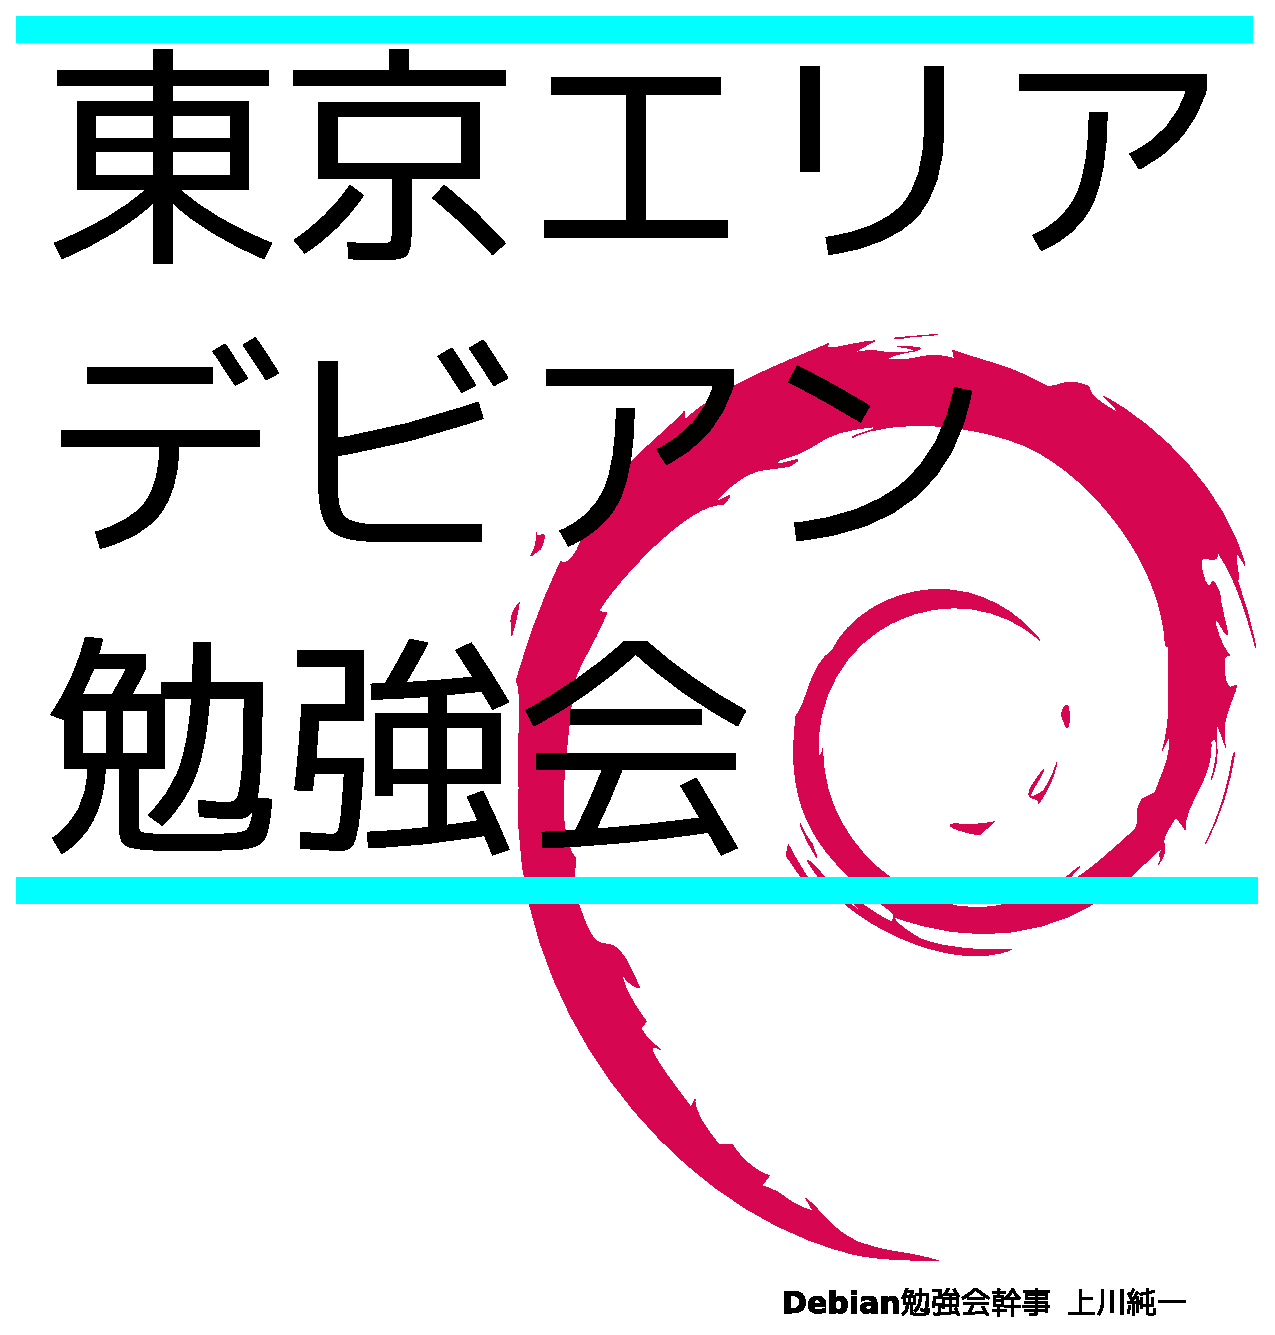
\includegraphics[width=210mm]{image200801/2008title.eps}\\
\hfill{}\debmtgyear{}$BG/(B\debmtgmonth{}$B7n(B\debmtgdate{}$BF|(B

\end{titlepage}

\dancersection{Introduction}{$B>e@n(B $B=c0l(B}

\begin{multicols}{2}
 
 
 $B:#7n$N(BDebian$BJY6/2q$X$h$&$3$=!#$3$l$+$i(BDebian$B$N@$3&$K$"$7$rF'$_F~$l$k$H(B
 $B$$$&J}$b!"$9$G$K$I$C$W$j$H$D$+$C$F$$$k$H$$$&J}$b!"7n$K0l2s(BDebian$B$K$D$$(B
 $B$F8l$j$^$;$s$+!)(B

 Debian$BJY6/2q$NL\E*$O2<5-$G$9!#(B

 \begin{itemize}
 \item \underline{Debian Developer} ($B3+H/<T(B)$B$N0i@.!#(B
 \item $BF|K\8l$G$N!V(B\underline{$B3+H/$K4X$9$k>pJs(B}$B!W$r@0M}$7$F$^$H$a!"%"%C%W%G!<%H$9$k!#(B
 \item \underline{$B>l(B}$B$NDs6!!#(B
 \begin{itemize}
  \item $BIaCJ$P$i$P$i$J>l=j$K$$$k?M!9$,(B face-to-face $B$G=P2q$($k>l$rDs6!(B
	$B$9$k!#(B
  \item Debian $B$N$?$a$K$J$k$3$H$r8l$k>l$rDs6!$9$k!#(B
  \item Debian$B$K$D$$$F8l$k>l$rDs6!$9$k!#(B
 \end{itemize}
 \end{itemize}		

 Debian$B$NJY6/2q$H$$$&$3$H$G5f6KE*$K$O;22C<TA40w$,(BDebian Package$B$r$,$j$,$j(B
 $B$H:n$k%9!<%Q!<%O%C%+!<$K$J$C$?;Q$rLQA[$7$F$$$^$9!#>pJs$N6&M-!&3hMQ$rDL$7(B
 $B$F(B Debian$B$N:#8e$NG=F0E*$JE83+$X$NEZBf$H$7$F!"!V>l!W$H$7$F$N6u4V$rDs6!$9(B
 $B$k$N$,L\E*$G$9!#(B

 2009$BG/$N7W2h$O2>$G$9!#(B

 \begin{enumerate}
  \item $B?7G/$N4k2h(B ($B%"%s%5%s%V%k2.7&3+:E(B)
  \item OSC Tokyo
  \item VAIO P $B%$%s%9%H!<%k5-O?!"(B
	$B%+!<%M%kFI=q2q!!%G%#%9%H%j%S%e!<%7%g%sBg=89g(B($B>.NS$5$s(B)($BEl5~Bg3X(B?)
  \item Git Handson ($B4d>>(B)($B$"$s$5$s$V$k2.7&(B?)
  \item $B2H(BDebian$B%5!<%P(B vs $B?&>l$N%M%C%H%o!<%/(B($B@iBeED6hETN)?^=q4[(B?\footnote{\url{http://www.library.chiyoda.tokyo.jp/}})
  \item Asterisk ($BEl5~Bg3X(B?)
  \item $B%9%Z%$%s$K$F3+:E(B
  \item Debconf$BJs9p2q(B
  \item OSC Fall?
  \item udev + HAL($B4d>>$5$s(B)
  \item 3D graphics $B3+H/!JF#Bt$5$s!K(B 
  \item Debian $B%5!<%P(B+VMware + $B3F<o(BOS$B!"(B
	$BB>$N2>A[2=%D!<%k(B(vserver etc.)$B!"(B
	$BK:G/2q(B
 \end{enumerate}

 $B2q>l8uJd$H$7$F$O2<5-$,$"$j$^$9(B:

 \begin{itemize}
  \item $BBg3X(B
  \item $B7CHf<w(BSGI$B%[!<%k(B
  \item Google$B%*%U%#%9(B
  \item $B8xL14[(B($B$"$s$5$s$V$k2.7&Ey(B)
  \item $BETN)2q5D<<(B($BL5@~(BLAN)
  \item $B7rJ]$N;\@_(B
 \end{itemize}

\end{multicols}


\newpage

\begin{minipage}[b]{0.2\hsize}
 \definecolor{titleback}{gray}{0.9}
 \colorbox{titleback}{\rotatebox{90}{\fontsize{80}{80} {\gt $B%G%S%"%sJY6/2q(B} }}
\end{minipage}
\begin{minipage}[b]{0.8\hsize}
\hrule
\vspace{2mm}
\hrule
%
% there are too many entries in 200901, usually
% we have tocdepth=2.
%
\setcounter{tocdepth}{1}
\tableofcontents
\vspace{2mm}
\hrule
\end{minipage}

\dancersection{$B;vA02]Bj(B}{$B>e@n(B $B=c0l(B}

??

{\bf $BLdBj(B}

\begin{enumerate}
 \item xxx
\end{enumerate}

$B$3$N2]Bj$KBP$7$FDs=P$$$?$@$$$?FbMF$O0J2<$G$9!#(B

\begin{multicols}{2}
%; whizzy-master ../debianmeetingresume200903.tex
% 以上の設定をしているため、このファイルで M-x whizzytex すると、whizzytexが利用できます。

\begin{prework}{上川純一}
\preworksection{XXXX}

\end{prework}

% この上の部分に以下の内容を挿入する。
% \begin{prework}{名前}
% \preworksection{XXX}
% \preworksection{YYY}
% \end{prework}
%

\end{multicols}

% image200903/prework.tex $BFbIt$K%F%-%9%H$rDI2C$7$F$/$@$5$$!#(B
%
%

\dancersection{$B:G6a$N(BDebian$B4XO"$N%_!<%F%#%s%0Js9p(B}{$B>e@n(B $B=c0l(B}
\subsection{$BEl5~%(%j%"(BDebian$BJY6/2q(B48$B2sL\Js9p(B}
% (query-replace-regexp "<.*?>" "")
% (query-replace-regexp "^[	 ]\+" "")

\subsection{$BEl5~%(%j%"(BDebian$BJY6/2q(B49$B2sL\Js9p(B}
% (query-replace-regexp "<.*?>" "")
% (query-replace-regexp "^[	 ]\+" "")


\subsection{Ubuntu XXX}

$B$d$^$M$5$s$,=q$/(B?

\subsection{Linux Consortium 10 years event }

\url{http://www.debian.or.jp/blog/events/linuxconsortium10th.html}
$B$K$D$$$F$d$^$M$5$s$,=q$/(B?

% ===============================================================
\dancersection{$B%+!<%M%kFI=q2q!!%G%#%9%H%j%S%e!<%7%g%sBg=89g(B}{$B>.NS576)(B}
\index{kernel}
\index{SVM}
\index{distribution}
\index{$B$V$s$5$s(B@$BJ,;6(B}
% ===============================================================

%============================================================
\dancersection{advi$B$r%G%P%C%0$7$F$_$?(B}{$BF|HfLn(B $B7<(B}
\index{OCaml}
\index{TeX}
%============================================================

2008$BG/(B11$B7n$N(BLaTeX$B$r;H$C$?%O%s%:%*%s$G!"(Bwizzytex-mode$B$+$i;H$o$l$F$$$k(B
advi$B$,$H$-$I$-8G$^$C$F$7$^$&LdBj$K$D$$$FD4$Y$F$_$^$7$?!#(B

\subsection{advi$B$,$^$k(B?}

advi$B$O0l8+IaDL$N(BDVI viewer$B$J$N$G$9$,!"$J$<$+(BOCaml$B$H$$$&JQ$o$C$?8@8l$G<BAu$5$l$F$$$^$9!#(B
$B:#2s$O(Badvi$B$+$i8F$P$l$k(Bghostscript$B$,;_$^$C$F$$$k$i$7$$!"(B
$B$H$$$&$3$H$^$GJ,$+$C$F$$$k>uBV$+$iD4$Y;O$a$^$7$?!#(B

\subsection{$B$H$j$"$($:%"%?%j$r$D$1$k(B}

$B$H$j$"$($:!"LdBj$,5/$-$F$$$k%=!<%9$r<h$C$F$-$FE83+$7$F$_$^$9!#(B

\begin{commandline}
% apt-get  source advi
...
dpkg-source: extracting advi in advi-1.6.0
dpkg-source: info: unpacking advi_1.6.0.orig.tar.gz
dpkg-source: info: applying advi_1.6.0-13.diff.gz
% cd advi-1.6.0
% ls *.ml
addons.ml     drawimage.ml  font.ml            gs.ml             main.ml     search.ml      transimpl.ml
ageometry.ml  driver.ml     global_options.ml  gterm.ml          misc.ml     shot.ml        ttfont.ml
...
\end{commandline}

*.ml$B$H$$$&$N$,(BOCaml$B$N%=!<%9%U%!%$%k$G$9!#$J$s$+!"(Bgs.ml$B$H$+$$$&$=$N$b$N%:%P%j$C$]$$$b$N$,8+$($^$9!#(B
gs.ml$B$NCf$r$^$:(Bgs$B$G8!:w$7$F$$$C$F$_$k$H!"(B

\begin{commandline}
...
  let command = Config.gs_path in
  let command_args =
    [|
      command; 
      "-dNOPLATFONTS"; "-dNOPAUSE";
      "-sDEVICE=" ^ (if !antialias then x11alpha else x11);
      "-q";
      "-dSAFER";
      "-";
    |] in

  let _ = debugs command;
...
\end{commandline}

$B$*$*!"$=$l$C$]$$!#$"$H!"%G%P%C%0MQ$C$]$$5!G=(B - debugs $B$rH/8+!#(B
$B$5$i$K$3$s$I$O(Bcommand$B$GC5$7$F$$$/$H!"(B

\begin{commandline}
...
  let lpd_in, lpd_out = Unix.pipe () in
...
  let leftout = Unix.out_channel_of_descr lpd_out in
...
  let pid =
    Unix.create_process command command_args lpd_in rpd_out
      (* Unix.stdout *) Unix.stderr
...
    method line l =
      try
        showps l;
        output_string leftout l;
        output_char leftout '\n';
...
\end{commandline}

$B$I$&$d$i(Bgs$B$K%Q%$%W$G(BPS$B$r=q$-$3$s$G$$$k$h$&$G$9!#(B
showps $B$H$+$$$&$N$G(BPS$B$NCf?H$r8+$k$3$H$,$G$-$k$s$8$c$J$$$+$J!<$H$+!#(B

\subsection{$B$^$8$a$KD4$Y$F$_$?$s$G$9$,(B...}

$B$b$&0lEY!"$3$s$I$O(Bgs.ml$B$N:G=i$NJ}$+$i%G%P%C%0MQ$N5!G=$@$18+$F$$$-$^$9!#(B

\begin{commandline}
...
let debugs = Misc.debug_endline;;
...
let showps_ref = ref false;;
let showps s =
  if !showps_ref then (print_endline  (Printf.sprintf "%s" s));;
...
Options.add
  "--showps" (Arg.Set showps_ref)
  "  ask advi to print to stdout a copy\
  \n\t of the PostScript program sent to gs.";;
...
\end{commandline}

\verb|Misc.| $B$H$$$&$N$O(B Misc$B$H$$$&JL$N%b%8%e!<%k$X$N;2>H$G$9!#$3$3$G$OC1$K(Bmisc.ml$B$NCf$r8+$l$P$h$5$=$&$G$9!#(B
\verb|showps_ref|$B$O=q$-49$(2DG=$J%U%i%0$N$h$&$G$9!#(B
$B$H;W$C$?$i$9$02<$K%3%^%s%I%i%$%s0z?t$+$i%U%i%0$r%;%C%H$G$-$k$h$&$K$J$C$F$$$k$h$&$G$9!#(B
misc.ml$B$NCf$b8+$F$_$k$H!"(B

\begin{commandline}
...
(* Debugging. *)
let forward_debug_endline =
  ref (function (_ : string) -> failwith "undefined forward debug_endline");;

let debug_endline s = (!forward_debug_endline s : unit);;

let set_forward_debug_endline f = forward_debug_endline := f;;
...
\end{commandline}

$B$5$i$K(B\verb|set_forward_debug_endline|$B$G(Bgrep$B$9$k$H!"(B\verb|global_options.ml|$B$,0z$C$+$+$k$N$G!"$=$NCf$b8+$F$_$k$H(B

\begin{commandline}
...
(* To print debugging messages. *)
let debug_endline = Options.debug "--debug" " General debug";;

(* Setting the forward in Misc. *)
Misc.set_forward_debug_endline debug_endline;;
...
\end{commandline}

$B7k6I!"$I$C$A$b%3%^%s%I%i%$%s$+$i@_Dj$G$-$k$h$&$G$9$M!#(B
$B$5$C$=$/;n$7$F$_$k$H!"(B

\begin{commandline}
% platex debianmeetingresume200812-presentation.tex
...
% advi debianmeetingresume200812-presentation.dvi
...
/usr/bin/gs
-dNOPLATFONTS
-dNOPAUSE
-sDEVICE=x11
-q
-dDELAYSAFER
-
...
%!PS-Adobe-2.0
%%Creator: Active-DVI
%!
[1 0 0 -1 0 0] concat
(/usr/share/texmf-texlive/dvips/base/texc.pro) run
(/usr/share/texmf-texlive/dvips/base/special.pro) run
...
%% Newpage

grestore
0 0 moveto
TeXDict begin 12769384 12769384 div dup /Resolution X /VResolution X end
TeXDict begin /DVImag 194.845342 def end
gsave
flushpage (...
) print flush 
\end{commandline}

$B$?$7$+$K(Bgs$B$N%3%^%s%I%i%$%s$i$7$-$b$N$H!"$=$l$+$i=q$-$3$s$@(BPS$B$NFbMF$i$7$$$b$N$,8+$($F$^$9!#(B
PS$B$GL\0u$H$J$kJ8;zNs$r=PNO$5$l$kL?Na(B \verb|flushpage (...) print flush| $B$r(Bgs$B$K=q$-$3$s$G!"(B
$B$=$N=PNO$rBT$C$F$$$k$h$&$J$N$G$9$,!"La$C$F$-$F$$$J$$$h$&$G$9!#(B

gs$B$,;_$^$C$F$7$^$&>l9g$H$=$&$G$J$$>l9g$bHf$Y$F$_$?$N$G$9$,!"(B
$B;_$^$C$F$7$^$&>l9g$N(BPS$B$N:G>.%;%C%H$r3d$j=P$9$N$,Fq$7$/!"$h$/$o$+$j$^$;$s$G$7$?!#(B

\subsection{$BJL$N2sHr:v(B?}

$B$J$K$+JL$NJ}K!$G;_$^$C$F$7$^$&$N$r2sHr$G$-$J$$$+!"$H(Bgs$B$N=PNO$rBT$C$F$$$kItJ,$b8+$F$_$^$9!#(B

\begin{commandline}
...
let rec select fd_in fd_out fd_exn timeout =
  (* dirty hack: Graphics uses itimer internally! *)
  let start = Unix.gettimeofday () in
  try
    Unix.select fd_in fd_out fd_exn timeout
  with
    Unix.Unix_error (Unix.EINTR, _, _) as exn ->
      let now = Unix.gettimeofday () in
      let remaining = start +. timeout -. now in
      if remaining > 0.0 then select fd_in fd_out fd_exn timeout else [], [], []
...
      match select [ rpd_in ] [] [] 1.0 with
      | [], _, _ ->
          begin match Unix.waitpid [ Unix.WNOHANG ] pid with
          | x, Unix.WEXITED y when x > 0 ->
              raise (Killed "gs exited")
          | 0, _ ->
              raise (Killed "gs alive but not responding")
          | _, _ ->
              raise (Killed "gs in strange state")
          end
...
\end{commandline}

gs$B$N=PNO$r(Bselect$B$GBT$C$F$$$k$h$&$G$9!#%?%$%`%"%&%H$b;E9~$s$G$"$k$h$&$G$9!#(B
$B$J$<$&$^$/$$$C$F$$$J$$$N$G$7$g$&!#(B

$B$3$3$G$OA0H>$GDj5A$5$l$F$$$k(Bselect$B$KCmL\$G$9!#(B
$B$;$C$+$/%?%$%`%"%&%H$N;D$j;~4V$r7W;;$7$F$$$k$N$K!"EO$7$F$$$k$N$O$b$H$NCM$G$9!#(B
$B$I$&$j$G$$$D$^$G$?$C$F$b%?%$%`%"%&%H$7$J$$$o$1$G$9!#(B

\begin{commandline}
...
if remaining > 0.0 then select fd_in fd_out fd_exn timeout else [], [], []
...
\end{commandline}

$B$3$l$r(B
\begin{commandline}
...
if remaining > 0.0 then select fd_in fd_out fd_exn remaining else [], [], []
...
\end{commandline}

$B$HD>$9$H!"(Bgs$B$rBT$C$F$b%?%$%`%"%&%H$9$k$h$&$K$J$j$^$9!#(B
gs$B$,8G$^$k860x$r<h$j=|$/$h$&$J:,K\E*$J2r7h$O$G$-$^$;$s$G$7$?$,!"(B
$B$H$j$"$($:$O(B advi $B$,;_$^$i$J$$$h$&$K$O$J$j$=$&$G$9!#(B

% ===============================================================
\dancersection{Debian on chumby$B$N:n$jJ}(B }{$B$^$($@$3$&$X$$(B}
\index{chumby}
\index{lenny}
\index{chroot}
% ===============================================================

OSC 2009 Tokyo/Spring$B$G$NEl5~%(%j%"(B Debian $BJY6/2q$N%V!<%9$G!"(BDebian on
chumby $B$r9T$$$^$7$?!#:#2s$O$=$N4D6-$N:n$jJ}$K$D$$$F$^$H$a$^$7$?!#(B
\begin{multicols}{2}
\subsection{$B35MW(B}
$B:#2s!"<B$O(Bchumby$B$N>e$G%M%$%F%#%V$K(BDebian$B$rF0$+$7$?$o$1$G$O$"$j$^$;$s!#(B
USB$B%a%b%j$K%$%s%9%H!<%k$7$?(BDebian$B$K(Bchroot$B$7$F5<;wE*$KF0$+$7$F$$(B
$B$k$h$&$K8+$;$+$1$^$7$?!#%M%$%F%#%V$KF0$+$9$H$J$k$H%V!<%H%m!<%@$r$$$8$kI,(B
$BMW$,$"$j$^$9$,!":#2s$O(Bchumby$B<+BN$O$[$H$s$IJQ99$;$:$K:Q$`J}K!$r$H$j$^$7$?!#(B

\subsubsection{chumby$B$N;EMM(B}
chumby$B$O!"%$%s%?!<%M%C%H$K@\B32DG=$JL5@~(BLAN$B4D6-$,I,MW$G!"@\B3$G$-$J(B
$B$1$l$P%"%J%m%0;~7W$N(Bwidget$B$NI=<($7$+$G$-$^$;$s!#$^$?!"=q$-9~$_2DG=$J%a%b(B
$B%jNN0h$O%U%i%C%7%e%a%b%j$b(B64MB$B$N$&$A!"$o$:$+$G$9(B\footnote{jffs2$B%U%!%$%k%7%9%F%`$G(B/psp$B$H$7$F%^%&%s%H$5$l$F$$$^$9!#(B}$B!#EvA3!"(BDebian$B$r%m!<%+%k$K%$%s%9%H!<%k$9$k$3$H$O$G$-$J$$$N$G!"(BUSB$B%a%b%j$r30It%9%H%l!<%8$H$7$F;H$$$^$9!#(B

$B$b$&0l$D$N@)Ls$O!"(Bchumby$B$O!"(Bext2$B$J$I$r;H$($^$;$s!#(BUSB$B%a%b%j$r;H$&>l9g$O(B
vfat$B$N$_$G$9!#$7$+$7(Bvfat$B$G$O(BLinux$B$r%$%s%9%H!<%k$G$-$^$;$s(B\footnote{$B860x(B
$B$O(Bsymlink$B$r:n@.$G$-$J$$$3$H!"E,@Z$J%Q!<%_%C%7%g%s$r@_Dj$G$-$J$$$3$H!"$J(B
$B$I!#(B}$B!#$=$3$G!"Bg$-$/#3$D$d$k$3$H$,$"$j$^$9!#(B
\begin{enumerate}
\item chumby$B$N%+!<%M%k%j%S%k%I(B
\item USB$B%a%b%j$X$N(BDebian$B%$%s%9%H!<%k(B
\item USB$B%a%b%j$N(BDebian$B$X$N(Bchroot$B@_Dj(B
\end{enumerate}
\subsection{$B4D6-9=C[(B}
\subsubsection{$BA0Ds>r7o(B}
\textbf{$B4D6-9=C[;~$K:GDc8BI,MW$J$b$N(B}
\begin{itemize}
\item chumby
\item USB$B%a%b%j(B
\item Debian$B4D6-9=C[MQ$N(BPC
\item $B%M%C%H%o!<%/4D6-(B
\end{itemize}
\subsubsection{chumby$B$N%+!<%M%k%j%S%k%I(B}
$BA0=R$N$H$*$j!"(Bchumby$B$N(Bkernel$B$O(Bext2$B$r;H$($^$;$s!#:#2s!"(BUSB$B%a%b%j$K$O(Bext2
$B%U%)!<%^%C%H$G(BDebian$B$r%$%s%9%H!<%k$9$k$N$G!"(Bchumby$B<+BN$b(Bext2$B$rFI$_9~$a$k(B
$B$h$&$K$7$^$9!#(B
$B$^$:!"2<5-%j%s%/@h$+$i(Bchumby$B$N%+!<%M%k9=C[MQ$N%D!<%k%-%C%H$rF~<j$7$^$9!#(B
$B<j=g$O%j%s%/@h$K=>$$$^$9!#(B
\begin{itemize}
\item GNU Toolchain\footnote{\url{http://wiki.chumby.com/mediawiki/index.php/GNU_Toolchain}}
\item GCC Toolchain\footnote{\url{http://wiki.chumby.com/mediawiki/index.php/GCC_Toolchain}}
\end{itemize}
$B$3$l$i$N%D!<%k%-%C%H$O!"(B/usr$B0J2<$KE83+$5$l$k$N$G!"(Bkvm/qemu$B$J$I$N2>A[(BOS$B4D(B
$B6-$K!"4D6-$r9=C[$9$k$HNI$$$G$7$g$&!#(B
\begin{commandline}
$ cd /
$ sudo tar zxf ~/arm-linux-v4.1.2b.tar.gz
$ sudo tar zxf ~/Gcc-3.3.2-glibc-2.3.2.tar.gz
$ sudo mkdir -p /opt/Embedix/usr/local/arm-linux
$ sudo ln -s /usr \
 /opt/Embedix/usr/local/arm-linux/gcc-3.3.2-glibc-2.3.2
$ sudo vi /usr/bin/arm-linux-make
$ sudo chmod +x /usr/bin/arm-linux-make
\end{commandline}
/usr/bin/arm-linux/make$B$K$O0J2<$N$h$&$K5-=R$7$^$9!#(B
\begin{commandline}
#!/bin/sh
echo make ARCH=arm CROSS=arm-linux- CC=arm-linux-gcc \
 AR=arm-linux-ar NM=arm-linux-nm RANLIB=arm-linux-ranlib \
 CXX=arm-linux-g++ AS=arm-linux-as LD=arm-linux-ld \
 STRIP=arm-linux-strip BUILDCC=gcc BUILD_CC=gcc \
 CC_FOR_BUILD=gcc ``$@''
exec make ARCH=arm CROSS=arm-linux- CC=arm-linux-gcc \
 AR=arm-linux-ar NM=arm-linux-nm RANLIB=arm-linux-ranlib \
 CXX=arm-linux-g++ AS=arm-linux-as LD=arm-linux-ld \
 STRIP=arm-linux-strip BUILDCC=gcc
 BUILD_CC=gcc CC_FOR_BUILD=gcc ``$@''
\end{commandline}
$B;d$N(Bchumby$B$N%U%!!<%`%&%'%"$O(B1.6\footnote{$B3NG'J}K!$O!"(Bssh$B$G(Bchumby$B$K%m%0%$(B
$B%s8e!"(Bchumby\_version -f$B$r<B9T$7$^$9!#(B}$B$J$N$G!"(BWiki$B$N(Bfirmware 1.6$B$N<j=g$r<B;\$7(B
$B$^$9!#(B
\begin{itemize}
\item Hacking Linux for chumby - ChumbyWiki\footnote{\url{http://wiki.chumby.com/mediawiki/index.php/Hacking_Linux_for_chumby}}
\end{itemize}
$B$^$?!"%+!<%M%k%S%k%IMQ$N4D6-$K$O<!$N(BDebian$B%Q%C%1!<%8$O:GDc8BF~$l$F$*$/I,(B
$BMW$,$"$j$^$9!#(B
\begin{itemize}
\item make
\item gcc
\item libncurses5-dev
\item libncursesw5-dev
\item zip
\end{itemize}
$B$^$?!"(Bchumby$BMQ$N%+!<%M%k%=!<%9%3!<%I$H!"(Bchumby$B$X?7$7$$%+!<%M%k$r%$%s%9%H!<%k$9(B
$B$k$?$a$K%"%i%$%a%s%H$9$k(BPerl$B%9%/%j%W%H$r$=$l$>$l%@%&%s%m!<%I$7$F$*$-$^$9!#(B
\begin{itemize}
\item linux-2.6.16-chumby-1.6.0.tar.gz\footnote{\url{http://files.chumby.com/source/ironforge/build733/linux-2.6.16-chumby-1.6.0.tar.gz}}
\item align.pl\footnote{\url{http://files.chumby.com/source/ironforge/build396/align.pl}}
\end{itemize}

$B%+!<%M%k%=!<%9$rE83+$7!"(Bmake menuconfig$B$G(Bext2$B$rAH$_9~$_$^$9(B\footnote{$B%b(B
$B%8%e!<%k$K$7$F$b9=$$$^$;$s$,!"$=$N>l9g$O<jF0$G%+!<%M%k%b%8%e!<%k$r%m!<%I(B
$B$9$kI,MW$,$"$k$N$GLLE]$G$9!#(B}$B!#(B
\begin{commandline}
$ cd
$ mkdir kernel
$ cd kernel
$ cp ~/{align.pl,linux-2.6.16-chumby-1.6.0.tar.gz} ./
$ tar zxf linux-2.6.16-chumby-1.6.0.tar.gz
$ cd linux-2.6.16-chumby-1.6.0
$ ARCH=arm BOARD=mx21ads CROSS_COMPILE=arm-linux- \
 make menuconfig
$ ARCH=arm BOARD=mx21ads CROSS_COMPILE=arm-linux- make
$ perl ../align.pl arch/arm/boot/zImage
$ zip k1.bin.zip arch/arm/boot/zImage
\end{commandline}
$B$3$l$G!"(Bkernel/linux-2.6.16-chumby-1.6.0/$B%G%#%l%/%H%jD>2<$K!"(Bk1.bin.zip
$B$,@8@.$5$l$^$9!#$3$l$r(BUSB$B%a%b%j$N(Bvfat$BNN0h$K%3%T!<$7$^$9!#(B
\begin{commandline}
$ sudo mount -t vfat /dev/sda1 /media/usb
$ sudo mkdir /media/usb/update2
$ sudo cp -i k1.bin.zip /media/usb/update2/
$ sudo umount /media/usb
\end{commandline}
chumby$B$r(Bspecial option mode$B$G5/F0$7!"(Bkernel$B$r%"%C%W%G!<%H$7$^$9!#(B
\begin{enumerate}
\item chumby$B$NEE8;$r(BOFF$B$K$7$?>uBV$G(BUSB$B%a%b%j$rA^$7$^$9!#(B
\item $B%?%C%A%9%/%j!<%s$r2!$7$?$^$^!"EE8;$rF~$l$k!#ESCf$G2!$7$?$^$^$K$9$k(B
      $B$H(Bspecial option mode$B$K$J$k$h!"$HI=<($5$l$k$N$G$=$N$^$^2!$7$D$E$1(B
      $B$^$9!#(B
\item special option mode$B$N%a%K%e!<2hLL$G(B''install updates''$B$r%/%j%C%/$7(B
      $B$^$9!#(B
\item ``Install from USB flash drive''$B$r%/%j%C%/$9$k$H!"(Bkernel$B$,%"%C%W%G!<(B
      $B%H$5$l!"<+F0E*$K:F5/F0$5$l$^$9!#(B
\end{enumerate}
\subsubsection{USB$B%a%b%j$X$N(BDebian$B%$%s%9%H!<%k(B}
$B<!$K!"(BUSB$B%a%b%j$K(BDebian$B$r%$%s%9%H!<%k$7$^$9$,!"(BUSB$B%a%b%j$K$O(Bchumby$B<+BN$N@_(B
$BDj$r9T$&$?$a$N%U%!%$%k$rCV$/(Bvfat$BNN0h$bI,MW$J$N$G!"(Bfdisk$B%3%^%s%I$G(B
/dev/sda1$B$r(Bvfat$B!"(B/dev/sda2$B$r(BLinux$BMQNN0h$r:n$j!"(Bmkfs$B%3%^%s%I$G%U%!%$%k%7(B
$B%9%F%`$r:n@.$7$F$*$-$^$9!#(B
\begin{commandline}
$ sudo fdisk /dev/sda
$ sudo mkfs.vfat /dev/sda1
$ sudo mke2fs    /dev/sda2
\end{commandline}
$B$3$N(Bsda2$B$NJ}$K!"(BDebian$B$r%$%s%9%H!<%k$7$^$9!#(Bchumby$B$O!"(BEABI(armel)$B$G$O$J(B
$B$/!"(BOABI(arm)$B$G$"$k$?$a!"(Barm$BHG$N%$%s%9%H!<%i$rMQ0U$9$kI,MW$,$"$j$^$9!#$7(B
$B$+$7!"(BQemu$B$G$O(Barmel$B$N%5%V%"!<%-%F%/%A%c(Bversatile$B$7$+%5%]!<%H$7$F$$$J$$$?(B
$B$a!"(Barm$BHG$N(Bkernel$B%$%a!<%8$r5/F0$5$;$k$3$H$7$+$G$-$^$;$s!#$J$N$G!":#2s$O!"(B
$BF1$8(BOABI$B$N%"%C%H%^!<%/%F%/%N<R$N(Barmadillo-9$BMQ$K8x3+$5$l$F$$$k(BDebian Etch$B%$%a!<(B
$B%8$rMxMQ$7$^$7$?!#2<5-%j%s%/@h$+$i!"(B5$B$D$N(Btar$B%\!<%k$rA4$F%@%&%s%m!<%I$7$^$9!#(B
\begin{itemize}
 \item debian directory - Armadillo $B3+H/<T%5%$%H(B\footnote{\url{http://armadillo.atmark-techno.com/filebrowser/armadillo-9/debian}}
\end{itemize}
ext2$BNN0h$r%^%&%s%H$7!"(Btar$B%\!<%k$rE83+$7$^$9!#(B
\begin{commandline}
$ sudo mount /dev/sda2 /mnt
$ cd /mnt
$ tar zxf ~/debian-etch-a9-1.tgz
$ tar zxf ~/debian-etch-a9-2.tgz
$ tar zxf ~/debian-etch-a9-3.tgz
$ tar zxf ~/debian-etch-a9-4.tgz
$ tar zxf ~/debian-etch-a9-5.tgz
\end{commandline}
chumby$B$NEE8;$rMn$H$7!"$3$N(BUSB$B%a%b%j$rA^$7$FEE8;$rF~$l$k$H!"<+F0E*$K(Bext2
$BNN0h$b%^%&%s%H$5$l!"$3$N2<$NNN0h$N%P%$%J%j$b@5>o$K<B9T$G$-$^$9!#(B
\subsubsection{USB$B4D6-$X$N(Bchroot$B=`Hw(B}
USB$B%a%b%j$N(BDebian$B4D6-$K(Bchroot$B$7!"$=$7$F$=$N4D6-2<$G(BEtch$B$+$i(BLenny$B$K%P!<(B
$B%8%g%s%"%C%W$5$;$^$9!#$^$:!"(Bssh$B$G%m%0%$%s$7!"(B/proc$B!"(B/dev$B!"(Bdevpts$B$r%P%$%s%I$5$;(B
$B$^$9!#(B
\begin{commandline}
chumby:~# mount -o bind /proc /mnt/usb2/proc
chumby:~# mount -o bind /dev  /mnt/usb2/dev
chumby:~# mount -t devpts devpts /mnt/usb2/dev/pts/
chumby:~# chroot /mnt/usb2
chumby:/1 df
Filesystem    1K-blocks      Used Available Use% Mounted on
/dev/hda1       1373548    181321   1118946  14% /
tmpfs           1373548    181321   1118946  14% /lib/init/rw
sysfs           1373548    181321   1118946  14% /sys
udev            1373548    181321   1118946  14% /dev
tmpfs           1373548    181321   1118946  14% /dev/shm
devpts          1373548    181321   1118946  14% /dev/pts
\end{commandline}
apt line$B$r(Betch$B$+$i(Blenny$B$K=q$-49$(!"%P!<%8%g%s%"%C%W$r9T$&$H!"LdBj$J$/%"%C(B
$B%W%0%l!<%I$G$-$k$O$:$G$9!#(B

$B<!$K!"(Bchroot$B$N(BDebian$B$G!"(Bssh$B$r<+F05/F0$5$;$k$?(B
$B$a!"<!$N@_Dj$r9T$$$^$9!#(B22/tcp$B$O(Bchumby$B<+BN$N(Bsshd$B$,;H$&$N$GJL$N%]!<%H$r3d(B
$B$jEv$F$kJ}$,NI$$$G$7$g$&!#(B

\textbf{/mnt/usb2/etc/ssh/sshd\_config ($B0lItH4?h(B)}
\begin{commandline}
Port 2222
(snip)
PermitRootLogin no
StrictModes yes
RSAAuthentication yes
PubkeyAuthentication yes
(snip)
PermitEmptyPasswords no
ChallengeResponseAuthentication no
PasswordAuthentication no
(snip)
\end{commandline}
$B<!$K!"(Bchumby$BB&$N@_Dj!#(BUSB$B%a%b%j$KG[CV$7$?(BWidget$B$r%m!<%I$5$;$k<j=g$N1~MQ(B
$B$G!"(B6.2.3$B$G:n@.$7$?(Bvfat$BNN0h$ND>2<$K!"0J2<$NFbMF$G(Bdebugchumby$B$H$$$&%U%!%$(B
$B%kL>$G%9%/%j%W%H$r:n@.$7$^$9!#(B
\begin{commandline}
#!/bin/bash

mount -o bind /proc /mnt/usb2/proc
mount -o bind /dev  /mnt/usb2/dev
mount -t devpts devpts /mnt/usb2/dev/pts/
chmod 666 /mnt/usb2/dev/null
chroot /mnt/usb2 /bin/hostname chumby
chroot /mnt/usb2 /usr/sbin/sshd
\end{commandline}
$B$3$l$G!"<!2s0J9_!"<+F0E*$K(Bchroot$B4D6-$N(BDebian$B$N(Bsshd$B$,(B2222/tcp$B$G5/F0$9$k$h(B
$B$&$K$J$j$^$9!#(B

\subsection{OSC$B2q>l$G$NE8<(=`Hw(B}
6.1$B$G$b=q$-$^$7$?$,!"(BChumny$B$O%$%s%?!<%M%C%H$K7R$,$i$J$$$HC1$J$k;~7W$G$9!#(B
$BM}M3$O!"5/F0;~$K(Bchumby.com$B$+$i(Bcontrolpanel.swf$B$H$$$&4IM}%3%s%=!<%k$N(B
flash$B%U%!%$%k$d!"$=$NB><+J,$G@_Dj$7$F$$$k(BWidget$B$r%@%&%s%m!<%I$7$F$/$k$?(B
$B$a$G$9!#$=$3$G!"4JC1$J(BWidget$B$r:n@.$7!"2hLL>e$O$=$l$rI=<($7$D$D!"%9%?%s%I(B
$B%"%m%s4D6-$G$bM-@~(BLAN$B$r2p$7$F(BSSH$B$G%m%0%$%s$G$-$k$h$&$K$7$^$9!#(B

\subsubsection{$BA0Ds>r7o(B}
\textbf{$B4D6-9=C[$K2C$($FI,MW$J$b$N(B}
\begin{itemize}
\item mtasc$B%Q%C%1!<%8(B
\item USB-Ethernet$BJQ49%"%@%W%?(B
\item $B%/%m%9%1!<%V%k(B
\item $BE8<(MQ$N(BPC
\end{itemize}

\subsubsection{Widget$B:n@.(B}
chumby$B$N(BWidget$B$O(BFlash$B$G$9!#(BDebian$B$r;H$C$F$$$k$N$G(BWidget$B$O$b$A$m$s%F%-%9(B
$B%H%(%G%#%?$G(BActionScript$B$r=q$$$F!"%U%j!<%=%U%H%&%'%"$G%3%s%Q%$%k$7$^$9!#(B
$B:#2s$NE8<($GI=<($5$;$F$$$?(BWidgit$B$N%=!<%9%3!<%I$O0J2<$N$H$*$j$G$9!#(B
\begin{commandline}
class DisplayDebian {
  public static function main(mc:MovieClip):Void
  {
    var app = new DisplayDebian(mc);
  }

  public function DisplayDebian(mc:MovieClip)
  {
    mc.createEmptyMovieClip(``image'',
    mc.getNextHighestDepth());
    var image:MovieClip = mc.image;
    var imageArr:Array = [ ``./openlogo.png'' ];
    image._xscale= 100;
    image._yscale= 100;
    image._x= 69;
    image._y= 0;
    image.loadMovie(imageArr[0]);

    var textField:TextField = mc.createTextField('textField',
    mc.getNextHighestDepth(), 15, 10, 320, 240);
    var fmt:TextFormat = new TextFormat('', 24, 0x000000);
    textField.text = '$BEl5~%(%j%"(B Debian $BJY6/2q(B\n\n\n' +
    '$B<!2s$O(B3/21,$BElBg$G3+:EM=Dj(B';
    textField.setTextFormat(fmt);
  }
}
\end{commandline}
$B$3$l$r(BHoge.as$B$H$7$FJ]B8$7!"F1$8%G%#%l%/%H%j$K(B
openlogo.png\footnote{Debian.org$B$N%5%$%H$N%m%4(B
\url{http://www.debian.org/logos/openlogo.xcf.gz}$B$rMxMQ!#$=$N$^$^$G$O2h(B
$BA|%5%$%:$,9g$o$J$$$?$a!"(Bgimp$B$G9b$5(B240$B%T%/%;%k$K<}$^$k$h$&$K%j%5%$%:$7$F(B
$B$$$^$9!#(B}$B$rG[CV$7$^$9!#(B

$B$=$7$F0J2<$N%o%s%i%$%J!<(B(ascompile.sh)$B$N0z?t$H$7$FEO$7!"%3%s%Q%$%k$7$^$9!#(B
\begin{commandline}
$ ./ascompile.sh Hoge.as
\end{commandline}
$B%o%s%i%$%J!<(Bascompile.sh$B$O0J2<$N$h$&$K5-=R$7$^$9!#(B
\begin{commandline}
#!/bin/bash
test -z $1 && exit 1
mtasc -swf `basename $1 .as`.swf -main $1 -header \
 320:240:12 -version 8
\end{commandline}
$B%3%s%Q%$%k$9$k$H!"(BHoge.swf$B$H$$$&(Bflash$B%U%!%$%k$,$G$-$^$9!#$3$N(BHoge.swf$B$r(B
Widget$B$H$7$FFI$_9~$`$?$a$K!"(Bprofile.xml$B$H$$$&L>A0$G@_Dj$7$^$9!#(B

\begin{commandline}
<?xml version=''1.0'' encoding=''utf-8'' ?>
<profile>
 <widget_instances>
  <widget_instance id=''1''>
   <widget>
    <name>Debian Logo</name>
    <description>Debian GNU/Linux Logo</description>
    <version>1.0</version>
    <mode time=''30'' mode=''timeout'' />
    <access sendable=''false'' deletable=''false''
     access=''private'' virtualable=''false'' />
    <user username=''Kouhei Maeda'' />
    <thumbnail href=''file:////mnt/usb/openlogo.png''
     contenttype=''image/png'' />
    <movie href=''file:////mnt/usb/Hoge.swf''
     contenttype=''application/x-shockwave-flash'' />
   </widget>
   <access access=''private'' />
   <mode time=''30'' mode=''timeout'' />
   <widget_parameters>
    <widget_parameter>
     <name>auther1</name>
     <value>Kouhei</value>
    </widget_parameter>
    <widget_paramter>
     <name>auther2</name>
     <value>Maeda</value>
    </widget_parameter>
   </widget_parameters>
  </widget_instance>
 </widget_instances>
</profile>
\end{commandline}
$B$3$N(Bprofile.xml$B$*$h$S!"(BHoge.swf$B$H(Bopenlogo.png$B$r(BUSB$B%a%b%j$N(Bvfat$BNN0hD>2<(B
$B$K%3%T!<$7$^$9!#$3$l$G!"5/F0;~$K(BUSB$B%a%b%j$+$i$3$N(BWidget$B$,FI$_9~$^$l$k$h(B
$B$&$K$J$j$^$9!#(B

\subsubsection{$B%9%?%s%I%"%m%s$G$N5/F0@_Dj(B}
$B<!$K!"%9%?%s%I%"%m%s$G@h$[$I$N(BWidget$B$,FI$_9~$^$l!"(Bssh$B$G%m%0%$%s$G$-$k$h(B
$B$&$K$7$^$9!#4pK\E*$K$O%U%)!<%i%`(B
\footnote{\url{http://forum.chumby.com/viewtopic.php?pid=12258}}$B$NFbMF$K(B
$B=>$C$F9T$($PLdBj$"$j$^$;$s!#(B
$B$^$:!"(B
chumby-offline.zip\footnote{\url{http://stud3.tuwien.ac.at/~e9825447/chumby-offline.zip}}
$B$r%@%&%s%m!<%I$7$^$9!#E83+$9$k$H(Boffline-howto.txt$B$H$$$&%I%-%e%a%s%H$,$"(B
$B$k$N$G!"$3$l$K=>$$@_Dj$7$^$9!#(Bprofile.xml$B$O4{$K(B6.3.2$B$G:n@.$7$F$$$^$9$N$G!"(B
$B$3$l$rMxMQ$7$F$/$@$5$$!#(BUSB$B%a%b%j$N(Bvfat$BNN0h$ND>2<$K0J2<$N%U%!%$%k$r%3%T!<(B
$B$7$^$9!#(B
\begin{itemize}
\item chumby-offline.zip$B$rE83+$7$F$G$-$k(Boffline$B%G%#%l%/%H%j0J2<$K$"$k(B
      www/$B%G%#%l%/%H%j(B\footnote{offline-howto.txt$B$K=>$$!"@_Dj:Q$_$G$"$k(B
      $B$3$H!#(B}
\item chumby$B$N(B/usr/widgets/controlpanel.swf
\end{itemize}
USB$B%a%b%j$N(Bvfat$BNN0h$ND>2<$N(Bdebugchumby$B$r<!$N$h$&$K=q$-49$($^$9!#(B
\begin{commandline}
#!/bin/bash

killall httpd
/usr/sbin/httpd -h /mnt/usb/www
cp /mnt/usb/www/hosts.offline /psp/hosts
#cp /mnt/usb/www/hosts.online /psp/hosts

mount -o bind /proc /mnt/usb2/proc
mount -o bind /dev  /mnt/usb2/dev
mount -t devpts devpts /mnt/usb2/dev/pts/
chmod 666 /mnt/usb2/dev/null
chroot /mnt/usb2 /bin/hostname chumby
\end{commandline}
$B$J$*!"%*%U%i%$%s%b!<%I$+$i%*%U%i%$%s%b!<%I$KLa$9>l9g$O!"(Bkillall$B$+$i#39T(B
$B$r%3%a%s%H%"%&%H$7!"(Bhosts.online$B$r%3%T!<$9$k9T$rM-8z$K$7$F$/$@$5$$!#(B

$B$=$7$F:G8e$K!"(BUSB-Ethernet$B%"%@%W%?$r;H$$!"M-@~(BLAN$B7PM3$G%"%/%;%9$G$-$k$h(B
$B$&$K@_Dj$7$^$9!#:#$^$G$HF1$8$/!"(Bvfat$BNN0h$K(Buserhook1$B$H$$$&%U%!%$%k$r:n@.(B
$B$7$^$9!#FbMF$O0J2<$N$H$*$j$G$9!#(B
\begin{commandline}
#!/bin/sh

USE_DHCP=0
IPADDR=192.168.3.10
NETMASK=255.255.255.0
GATEWAY=192.168.3.1

/sbin/insmod /drivers/usbnet.ko
/sbin/insmod /drivers/pegasus.ko

ifconfig rausb0 127.0.0.1

if [ $USE_DHCP == 1 ]\daggerhen
   udhcpc -t 5 -n -p /var/run/udhcpc.eth0.pid -i eth0
else
   /sbin/ifconfig eth0 $IPADDR netmask $NETMASK
   /sbin/route add default gw $GATEWAY eth0
fi 
\end{commandline}
$B$A$J$_$K!":#2s$O(BBUFFALO$B$N(BLUA2-TX$B$r;H$C$F$$$^$9!#(B\footnote{$B$3$l$N%G%P%$%9%I%i%$(B
$B%P$O(Bpegasus.ko$B$G$9!#(B}

$B0J>e$G!"$^$C$?$/%$%s%?!<%M%C%H$r;H$($J$$4D6-$G$b!"M-@~(BLAN$B7PM3$G(BSSH$B@\B3$+(B
$B$D!"1U>=%b%K%?>e$K(BUSB$B$KF~$l$?(BWidget$B$r2TF/$5$;$k$3$H$,$G$-$k$h$&$K$J$j$^(B
$B$9!#(B
\subsection{$B;D:n6H(B}
$B0J2<$,;D$C$F$$$^$9$,!"5$$,8~$$$?$i$d$k$+$b$7$l$J$$$7!"$d$i$J$$$+$b$7$l$^$;$s!#(B
\begin{itemize}
\item debootstrap$B$G(BLenny arm$BHG$r:n$C$F$_$F(Bchroot$B4D6-$H$7$F;H$($k$+!)(B
\item chroot$B4D6-$+$i%U%l!<%`%P%C%U%!$r>h$C<h$k!#(B
\item $B%V!<%H%m!<%@$r%O%C%/$7$F!"D>@\(BUSB$B%V!<%H$5$;$k!#(B
\end{itemize}
\subsection{$B$*$^$1!':#7n$N%h%aH,6l(B}
2$B7n$O$3$N(BOSC$B=`Hw$HJL7o$G!"%h%a$h$j$bAa$/5"$C$F$-$F$bHUHS$r:n$i$J$+$C$?(B
$B!J:n$l$J$+$C$?!K$N$H!"Kh=5?eMK$K(BHack Meeting$B$K;22C$9$k$h$&$K$J$C$?$?$a!"(B
$B$a$C$A$cIT5!7y$K$J$j$^$7$?!#%3%o!#J}!9$N%"%I%P%$%9$rD:$-!"#37n8=:_$O(B``$B$9(B
$B$$!A$D(B''$B$G$J$@$a$F$$$^$9!#(B

\subsection{$B;29MJ88%(B}
\begin{itemize}
\item chumby$B$GM7$\$&!*(B

6.3.2$B$N(BHoge.as$B$OK\=q$N(Bp.48-49$B$N(BMain.as$B$r!"(Bprofile.xml$B$O(Bp.53$B$N(BUSB$B%a%b%j(B
      $BMQ(Bprofile.xml$B$NNc$r!"(B6.3.3$B$N(Buserhook1$B$O(Bp.156$B$N(Buserhook1$B$r0zMQ$7$^(B
      $B$7$?!#!J0lIt%Q%i%a!<%?$rJQ99!K(B

\begin{itemize}
\item ISBN : 978-4-7973-5039-5
\item $BCx<T(B : $BJFED(B $BAo(B
\item $BH/9T=j(B : $B%=%U%H%P%s%/%/%j%(%$%F%#%V3t<02q<R(B
\end{itemize}
\item Using Chumby offline  - Chumbysphere Forum
\begin{itemize}
\item \url{http://forum.chumby.com/viewtopic.php?pid=12258}
\end{itemize}
\item Hacking Linux for chumby - ChumbyWiki
\begin{itemize}
\item \url{http://wiki.chumby.com/mediawiki/index.php/Hacking_Linux_for_chumby}
\end{itemize}
\end{itemize}
\end{multicols}


\clearpage

%\printindex

\cleartooddpage

\vspace*{15cm}
\hrule
\vspace{2mm}
\includegraphics[width=2cm]{image200502/openlogo-nd.eps}
\noindent \Large \bf Debian $BJY6/2q;qNA(B\\ \\
\noindent \normalfont \debmtgyear{}$BG/(B\debmtgmonth{}$B7n(B\debmtgdate{}$BF|(B \hspace{5mm}  $B=iHGBh(B1$B:~H/9T(B\\
\noindent \normalfont $BEl5~%(%j%"(B Debian $BJY6/2q(B $B!JJT=8!&0u:~!&H/9T!K(B\\
\hrule


\end{document}
